\documentclass[tikz,border=2pt]{standalone}
\usepackage{amsmath,amssymb}
\usepackage{tikz}
\usetikzlibrary{matrix,arrows.meta}

\begin{document}
% Subtracting a constant from a whole row (or column) lowers the cost of EVERY complete
% assignment by that constant, because each assignment uses exactly one entry of the row:
% the ranking of assignments, hence the optimum, is unchanged.
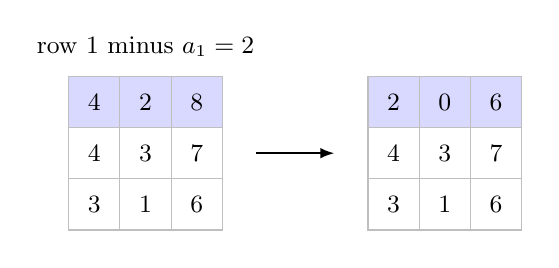
\begin{tikzpicture}[every node/.style={font=\small}, >={Latex[length=1.8mm]}]
	\matrix (A) [matrix of math nodes, nodes={minimum size=6.5mm, anchor=center, draw=gray!50}, column sep=-\pgflinewidth, row sep=-\pgflinewidth] at (0,0) {|[fill=blue!15]| 4 & |[fill=blue!15]| 2 & |[fill=blue!15]| 8 \\ 4 & 3 & 7 \\ 3 & 1 & 6 \\};
	\node[anchor=south] at (A.north) {row $1$ minus $a_1=2$};
	\draw[->, thick] (1.4,0) -- (2.4,0);
	\matrix (B) [matrix of math nodes, nodes={minimum size=6.5mm, anchor=center, draw=gray!50}, column sep=-\pgflinewidth, row sep=-\pgflinewidth] at (3.8,0) {|[fill=blue!15]| 2 & |[fill=blue!15]| 0 & |[fill=blue!15]| 6 \\ 4 & 3 & 7 \\ 3 & 1 & 6 \\};
	\end{tikzpicture}
\end{document}
